%% This is an example first chapter.  You should put chapter/appendix that you
%% write into a separate file, and add a line \include{yourfilename} to
%% main.tex, where `yourfilename.tex' is the name of the chapter/appendix file.
%% You can process specific files by typing their names in at the 
%% \files=
%% prompt when you run the file main.tex through LaTeX.

\singlespacing{

\chapter{Design Hierarchy}

with a scaling factor of about 100x between levels of hierarchy.

The details of the fabrication and joining strategies for these physical parts is beyond the scope of this thesis, though current ideas are briefly addressed here.  Initial thoughts about length scales are included here, but are meant only as a starting point for the 

\section{Elements}

At the lowest level, bulk materials in the form of \textit{elements} are assembled together to form multi-material assemblies.  Our notion of "element" is not an atomic element, but rather a homogenous volume of material with characteristic material properties.  A finite set of elemental types will be chosen based on desirable physical properties, cost, ease of fabrication, and compatibility with other elemental types and assembly processes.\\

For example, an aluminum element type would have the properties of being conductive, stiff, and lightweight and a rubber element type would be insulating and flexible.  Other element types of interest include magnetic and magnetically permeable types, silicon types, actuation types, and thermally conductive and insulating types.\\

Elemental components will be fabricated to a size on the order of ~1-10$\mu$m\textsuperscript{3}.  Some, as yet to be determined, form of joining interface must be incorporated into the geometry of the elemental parts or applied (in the form of an adhesive) to the parts during the assembly process.  This joining strategy may or may not be permanent.

\section{Functions}

Assemblies of elements form \textit{functions} - larger scale part types with material properties defined by their constituent elements.  As the name suggests, functions are categorized based on higher-level interactions with neighboring electro-mechanical systems, rather than their bulk material properties.  Function-level components fall into one of several functional archetypes, including but not limited to n-degree-of-freedom mechanical latches, hinges, and actuators, electronic memory storage, electronic oscillators, timers, and programmable logic.  Anisotropic patterns of elemental types within a function-level component may give the function tunable anisotropic behaviors.\\

Examples of function-level components would be routing components, which pass one or several electronic signals to neighboring components, or a one degree-of-freedom hinge, which displays low bending stiffness around one axis and high stiffness in the remaining directions.  This level of design hierarchy would grow to include actuators with tunable anisotropy, strain, and stress, and simple programmable silicon parts.  A more complete discussion of the diversity of mechanical part types at the function-level is given in Chapter \ref{chap:functionSim}.\\

Functional components will be on the order of ~1mm\textsuperscript{3}.  Some form of common interface must allow for both mechanical loads and analog electronic signals to pass from one function component to another.  At the function-level, a reversible joining interface is preferred so that reconfigurable behavior and recycling is possible.

\section{Modules}

\textit{Modules} are assemblies of function-level components, joined together to form robotic subsystems.  Modules combine electronic and mechanical functionality to achieve singular, high-level robotic tasks.  Modules will communicate with each other through an abstracted, digital interface.  Each module will own its own microprocessing unit that coordinates its function-level actuators and other active components.  This way, the low-level description of the structure within a module remains internal to the module itself.\\

Examples of modules include end effectors like grippers, clamping mechanisms, and sensors, actuation/locomotion systems, energy storage and generation, and large memory or programmable logic banks.  Joining interfaces between modules will allow mechanical forces, power, and a few digital signals to pass from one module to the next.  As with functions, modules should be reversibly joined.  The interface between modules may consist of many parallel function-level interfaces, or a bulk, module-level interface.\\

Modules will be built on the order of ~1cm\textsuperscript{3}.  Though modules may use mechanical compliance at the function-level to increase their internal degrees of freedom, at larger scales modules act as rigid bodies with internal motion.  That is, internal mechanical compliance within a module does not propagate to interactions with neighboring modules.  This idea follows from a model of how traditional solid-bodied rotary and linear actuators are viewed within a larger robotic structure.

\section{Complexes}

Assemblies of modules form \textit{complexes}, self-contained robotic systems that coordinate their own sensing, memory, logic, power, and/or actuation.  The key distinction between the module and complex-level is that complexes integrate inputs, outputs, logic, and memory, whereas modules specialize in only one of these tasks.  A complex could be a single, locomoting robot or manipulator, or an active, environmental system that performs sensing, actuation, or logical tasks across space.\\

Complexes will interact with function-level and module-level feedstock to accomplish assembly tasks.  shuttles materials across it (like a conveyor belt)\\

Complexes will be comprised of several to hundreds of individual modules, spanning length scales on the order of ten of cm to m.  Complexes should be considered independent, self-contained units.  The interface between complexes will be governed by end effector modules that the complex owns.

\section{Systems of Complexes}

Many complexes of various forms and functions may work together at a \textit{system}-level to accomplish large scale tasks.  More layers of hierarchy could be developed across this 

\section{Design Hierarchy in Biology}

\begin{sidewaysfigure}
  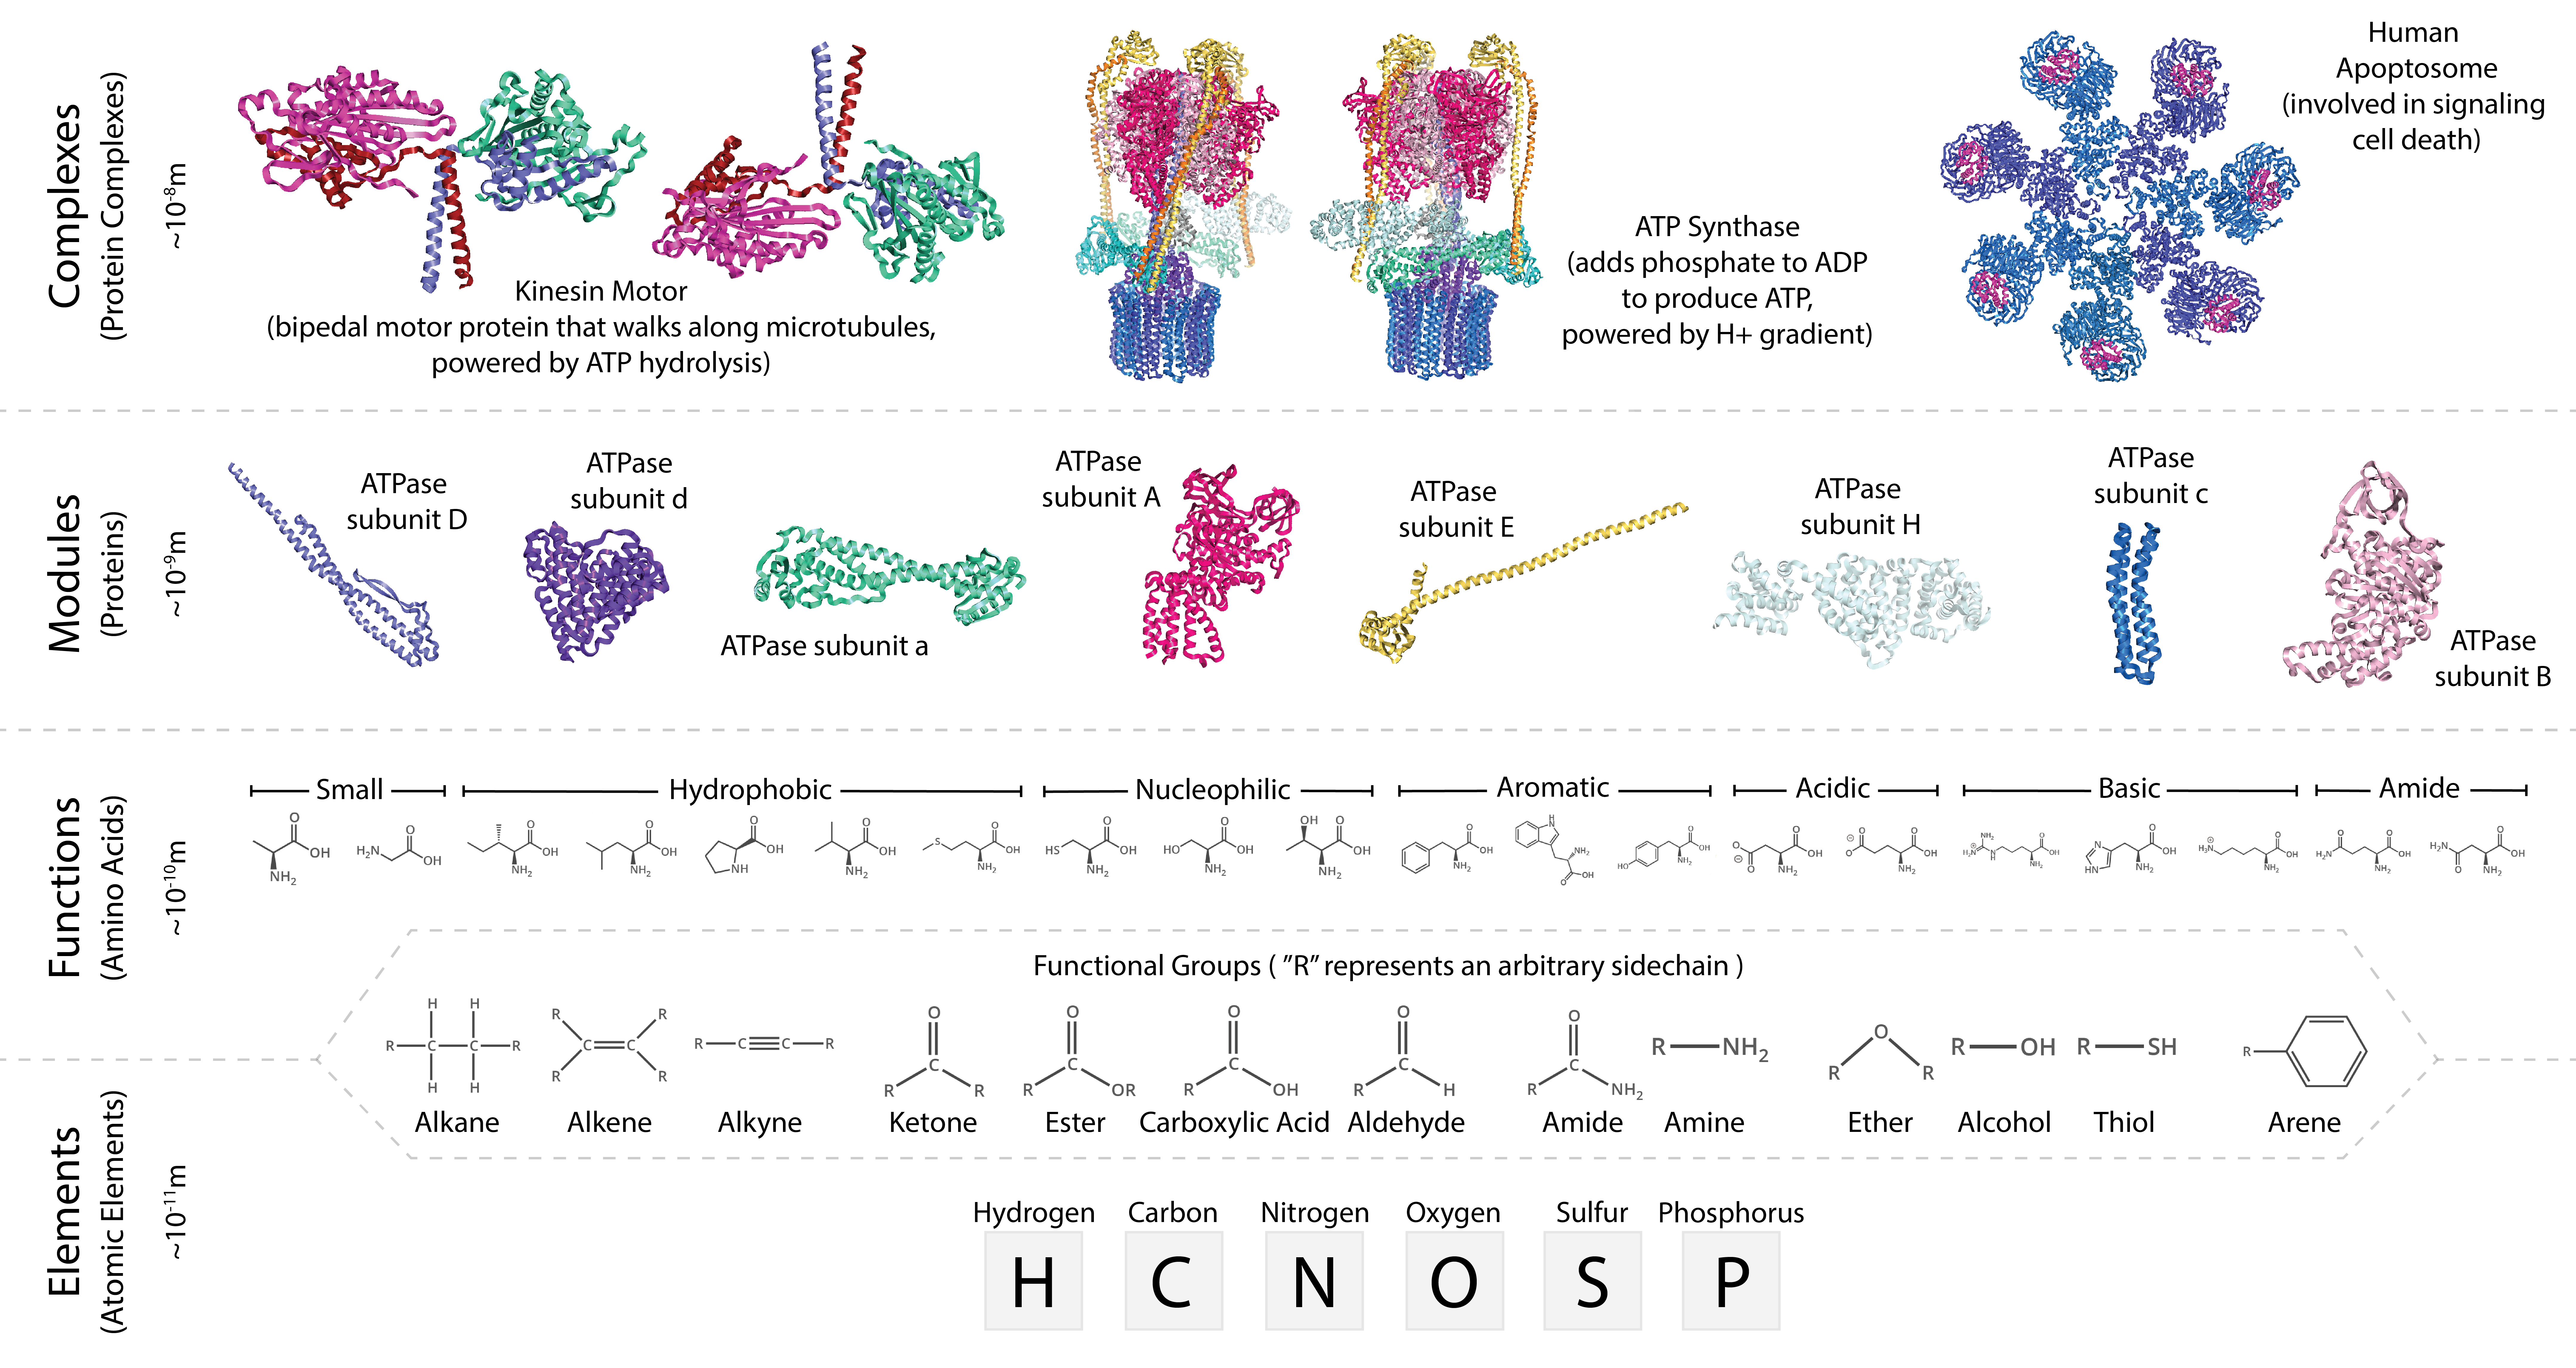
\includegraphics[width=\textwidth,height=\textheight,keepaspectratio]{ProteinHierarchy.png}
  \caption{Hierarchical breakdown of protein complexes (complexes) into proteins (modules), amino acids (functions), and atoms (elements).}
  \label{fig:ProteinHierarchy}
\end{sidewaysfigure}


Currently, the only known example of a physical, self-replicating system is the biology that has evolved on Earth.  Though we observe some slight variation across species, all biological self replication involves the use of protein machinery (called "protein complexes") built primarily from a small set of amino acid building blocks.\\

The construction of protein complexes takes place in a hierarchical fashion.  Figure \ref{fig:ProteinHierarchy} describes the hierarchical breakdown of protein complexes in terms of the four levels of hierarchy established earlier in this chapter; protein complexes (complex-level objects) are decomposed into proteins (modules), then into amino acids (functions), and finally into atomic elements (elements).  This hierarchical breakdown is slightly different from the primary/secondary/tertiary/quaternary structures typically used to discuss the levels of protein description.  The similarity of some of the biological nomenclature to our own hierarchical nomenclature is due to the fact that it was derived from the biological model.

\subsection{Elements, Functional Groups, and Functions}

At the most fundamental level, biological structures are composed of atoms of various elemental types.  Most biological molecules on Earth, especially those involved in protein synthesis and activation, are made from combinations of carbon, hydrogen, nitrogen, oxygen, phosphorus, and sulfur (CHNOPS).\\

Each element's unique position on the periodic table dictates its physical properties, which have implications in higher-level structures formed from the elements.  These properties include the element's mass, the number of covalent bonds it can form, the number of paired electrons it contains in its outermost electron shell, the polarization of the bonds and molecules it forms with other elements, and the stability of its bonds in various environments.\\

Certain motifs of covalently bonded atoms form \textit{functional groups} within molecules.  Functional groups determine the ability of a molecule to undergo various archetypal reactions (addition, substitution, elimination, etc) functional groups on other molecules.  A subset of the important functional groups found in biochemistry are indicated in Figure \ref{fig:ProteinHierarchy}.  "R" indicates an arbitrary side-chain, where the functional group connects to the rest of the molecule.\\

%In organic chemistry, the identification of functional groups allow us to abstract the interactions between molecules based on to predict how they will react in certain conditions.


\begin{figure}
  \includegraphics[width=\textwidth]{AminosInterface.png}
  \caption{(A) Decomposition of amino acids into carboxylic acid and amine interfaces and unique side-chain. (B) Formation of peptide bond at c-terminus (carboxylic acid group) of polypeptide chain with the n-terminus (amine group) of an amino acid. One molecule of water is produced as a byproduct of the peptide bonding reaction.  R, R', and R'' represent arbitrary amino acid side-chains.  Peptide bonds bolded.}
  \label{fig:AminosInterface}
\end{figure}

\textit{Amino acids} are molecules which contain several functional groups.  As indicated in Figure \ref{fig:AminosInterface}A all amino acids contain a carboxylic acid (COOH) and an amine group (NH\textsubscript{2} or NRH).  The purpose of these groups is to form the peptide bonds between amino acids in a polypeptide chain.  Peptide bonding forms a covalent bond between two amino acids through a process called "condensation", with a single molecule of water created as a byproduct \ref{fig:AminosInterface}B.\\

The remaining portion of an amino acid molecule (indicated by "R" in the amino acid archetype in Figure \ref{fig:AminosInterface}A, we'll call it "\textit{the} side-chain") determines its unique properties specific to each type of amino acid.  This side-chain may consist of one or more distinct functional groups.  Amino acids are characterized according to their side-chains in several ways; one grouping is shown in Figure \ref{fig:ProteinHierarchy}, with amino acids described by size, polarity, nucleophilicity, the presence of aromatic rings, acidity or basicity, and the presence of amide groups.\\

We can think of each of the amino acids as being composed of a standard interface and a unique, functional side-chain in the same way that our function-level engineered parts will be comprised of a standard interface and a unique, functional interior.  The carboxylic and amine groups common to all amino acids allow for polymerization along one dimension, and subsequent folding into three dimensions; we plan to design our interface to accommodate something analogous to "polymerization" in three dimensions.\\

 \subsection{Modules and Complexes}

Polypeptide chains typically consisting of hundreds of amino acids fold to form three dimensional \textit{proteins}.  

\subsection{Systems}

Beyond protein complexes, more levels of hierarchy exist within biological organisms to carry out systems-level tasks.  Protein complexes can be grouped according to the chemical pathways they interact with within a cell, by the organelles they belong to                                                                                                                                                                                                 

Organelles are organized within cells, cells within tissues, tissues within organs, organs within even higher level systems, and ultimately these systems come together in one complete organism.

\subsection{Scaling}

In the biological example, each level of hierarchy introduces a factor of about 10x in scaling.  The atoms that compose the lowest level of hierarchy have covalent diameters ranging from 50-200pm \cite{Slater1993}.  Amino acid diameters can be roughly calculated from atomic radii and three-dimensional structure to a range of 0.42-1.2nm \cite{Pool2003}.  The average protein length across prokaryotes and eukaryotes is about 200-400 amino acids, with a mass of about 20-40kDa \cite{Brocchieri2005}.  Assuming a simple spherical shape, this mass translates to a typical protein diameter of about 3-4nm \cite{Erickson2009}.  Known protein complexes are comprised of two to several hundred protein monomers with typical complex diameters ranging from about 8-100nm \cite{Yang2010a}.\\

Beyond these first four hierarchical levels, higher systems...
Assembly within is not carried out by a single protein complex, but rather, by the coordinated efforts of several complexes.

\subsection{Fabrication Insights}

synthesis of amino acids? recycling, breakdown to function level

\subsection{Combinatorial Design Space}

number of elements\\
number of amino acids - ribozyme, other species\\
number of protiens\\
number of complexes - design modularity\\

\section{Design Hierarchy in Conway's Game of Life}

In the 1940's Von Neumann began studying the requirements for self-replication and evolvability in artificial, CA worlds \cite{Neumann1966}.  One such world that has gained widespread notoriety is Conway's Game of Life ("Life").  Since it's inception in 1970, Life has developed a cult following of researchers, engineers, and hobbyists, pushing each other to construct increasingly elaborate "machines" from pixels on a screen.  These investigations have resulted in a lengthy taxonomy of motifs, reactions, mechanisms, and complex engineered systems within Life.  Some notable accomplishments include Gemini (an oblique spaceship encoded by a long glider tape)\cite{Wade2010}, the Linear Propagator (a self replicating machine)\cite{Greene2013}, a Universal Turing Machine \cite{Rendell2000}, and the OTCA Metapixel (a structure that behaves like a large-scale Life pixel)\cite{Due2006}.\\

The analogies between machines in Life and our proposed assembly system are limited, due to the fact that Life is inherently non-physical; it violates basic conservation principals, has no notion of cell joining, and is based on highly abstracted interactions.  However it provides an example of how engineered self-replication is possible using extremely simple building blocks, so-called "non-trivial" self-replication.  A proof of the existence of non-trivial self-replicating patterns in Life was first published by Conway, Berekamp, and Guy in 1982\cite{Berekamp1982}, and several decades later the first implementations of non-trivial replicators began emerging on online Life forums.  This work argues that the basic requirements for self-replication - universal computation and universal construction - are not only \textit{not} unique to biology, but are, in fact, quite prevalent in other virtual and physical systems.  An excellent analysis of Conway's existence proof, as well as an introduction to important concepts in Life can be found in \textit{The Recursive Universe} by William Poundstone\cite{Poundstone1985}.\\

\begin{figure}
  \includegraphics[width=\textwidth]{OTCAGalaxy.png}
  \caption{Nine timesteps of a 15x15 array of OTCA Metapixels playing out a period-8 oscillating pattern called "Kok's Galaxy".  Each timestep represents 35,328 generations of Life; the entire 8 step sequence takes 282,624 generations to complete.  Each metacell occupies 2058x2058 Life cells; the complete 15x15 metapixel array totals 30,800x30,800 Life cells (accounting for a 5 cell overlap between adjacent metacells).  10x magnification of a "living" and "dead" cell are shown at the top of the image.}
  \label{fig:OTCAGalaxy}
\end{figure}

In the next sections, I'll analyze a particularly complex Life pattern in terms of the hierarchies I introduced earlier in the chapter.  The OTCA Metapixel was designed by Brice Due in 2006\cite{Due2006}\cite{Ghassaei2015}.  Though not the first \textit{metacell} (a structure that can mimick a CA cell), it is the first \textit{metapixel} (a structure that looks and behaves like a macro-scale CA pixel) built in Life, and it can be programmed to perform any CA ruleset that's based on a summation of a cell's 8 local neighbors.  Many metapixels can be patterned together on a grid to play out a macro-scale CA (Figure \ref{fig:OTCAGalaxy}).

\subsection{Elements, Motifs, and Functions}

The first few levels of hierarchy within Life are illustrated in Figure \ref{fig:OTCAMetaHierarchy}.  At the most basic level, structures within Life are constructed from \textit{cells}.  Each cell is represented by one pixel on a Life grid and stores a binary state - "living" or "dead".  Cells interact with each other according to Conway's rules: living cells with 2 or 3 neighbors stay alive, dead cells with exactly 3 neighbors become living, and all other configurations die or stay dead.  Though the logic of cell-cell interactions is simple, the long term behavior of a given initial condition is often impossible to intuit. \\

Small assemblies of cells form \textit{motifs} on the order of about 5 cells across.  \textit{Still Lifes} are a category of motif that are static across generations unless acted upon by another pattern.  \textit{Oscillators} repeatedly morph between several conformations at some regular time interval.  Oscillators are categorized based on their period, for example, the Blinker and Beacon (Figure \ref{fig:OTCAMetaHierarchy}) are period-2 oscillators, and Kok's Galaxy (Figure \ref{fig:OTCAGalaxy}) is a period-8 oscillator.  \textit{Spaceships} are oscillators that move across the Life grid as they oscillate.  Gliders, the smallest type of spaceship in Life, move across space in diagonal directions (Figure \ref{fig:OTCAMetaHierarchy}).  Other spaceships, such as Light Weight, Medium Weight or Heavy Weight Spaceships (LWSS, MWSS, and HWSS, respectively) move in cartesian directions (Figure \ref{fig:OTCAMetaHierarchy}).  Spaceships are categorized based on their period and on their speed.  \textit{Methuselahs} are small patterns that take a large number of generations to eventually stabilize.  R-Pentamino is a Methuselah of only 5 initial cells that stabilizes in 1103 generations (Figure \ref{fig:OTCAMetaHierarchy}).\\

At the function-level, Life patterns on the scale of about 50 cells interact with each other in more structured and predictable ways.  In order for two function-level patterns to be compatible, their periods must have some common factor.  For example, period-4 LWSSes are compatible with 

\begin{sidewaysfigure}
  \includegraphics[width=\textwidth,height=\textheight,keepaspectratio]{OTCAMetaHierarchy.png}
  \caption{Hierarchical breakdown of OTCA Metapixel.}
  \label{fig:OTCAMetaHierarchy}
\end{sidewaysfigure}

\subsection{Modules and Complexes}

\begin{figure}
  \includegraphics[width=\textwidth]{OTCADiagram.png}
  \caption{Complex-level diagram of OTCA Metapixel with the most important modules highlighted.}
  \label{fig:OTCADiagram}
\end{figure}

\subsection{Scaling}

\subsection{Fabrication Insights}

\subsection{Combinatorial Design Space}

\section{Electronic Versus Mechanical Hierarchies}

scaling mismatch between the functional density of electronic and mechanical systems, offset in hierarchical setup.

\section{Hierarchy in Simulation}

increasing simulation abstraction as hierarchical level increases\\

In the next chapters, I'll describe the methods used to simulate assemblies of elements and functions, and describe how abstractions of the element-level simulation are adapted to the function-level.



}
